%\textit{% Szglab4
% ===========================================================================
%
\setcounter{chapter}{-1}
\chapter{Módosítások}

\section{Változások a specifikációban}

\subsection{Ragacs eltűnése}
\textbf{A ragacs eltűnik a pályáról, miután négy robot ráugrott (elkopik)}

Az Obstacle ősosztályban bevezettünk egy int típusú lifetime változót, amit a ragacs konstruktorában 4-re inicializálunk. Ha egy robot belelép a ragacsba, akkor ezt a változót eggyel csökkentjük, illetve ha elérte a 0-t, akkor értelemszerűen már nincs hatással a robotokra.

\subsection{Olaj felszáradása}
\textbf{Egy meghatározott idő letelte után az olajfolt eltűnik a pályáról (felszárad)}

Az említett lifetime változót az olaj konstruktorában 15-re inicializáljuk és mindig eggyel csökkentjük, amikor a robotok ugranak. Így 15 ugrás után már nem lesz hatással a robotokra, eltűnik.

\subsection{Tisztító kisrobotok}
\textbf{A pályára időnként keményen dolgozó kisrobotok jutnak be, akik szépen sorban feltakarítják a foltokat. A kisrobot egységnyi sebességgel halad, adott ideig (pl. két kör) takarítja a foltot. A folt feltakarítása után a legközelebbi folthoz indul. Ha egy robot ráugrik, akkor a kisrobot megsemmisül és olajfolt kerül a helyére; a ráugró robot nem szenved sérülést. Ha a kisrobot másik kisrobotnak vagy robotnak ütközik, irányt vált.}

Létrehoztunk egy új Cleaner osztályt, ami a Robotból származik le. Letiltottuk azokat az örökölt metódusokat, amik a tisztító robotra nem érvényesek. Ilyen páldául a setOiled() vagy setGlue(), hiszen a tisztító robotra ezek az akadályok nincsenek hatással. Mivel a tisztító robotnak tudnia kell, hogy melyik akadály van hozzá legközelebb, ezért egy tagváltozóként megkapja a pályán levő összes akadály listáját. Ezen a listán végigiterálva számolja ki az Obstacle visszatérésű nextObstacle() metódussal, hogy melyik folthoz induljon. Felül kellett definiálni a move() metódust, hiszen a kisrobot állapotától (mozog vagy takarít) függ, hogy hogyan viselkedik. Ha a kisrobot MOVING állapotban van, akkor folyamatosan kiszámolja, hogy melyik folt van hozzá a legközelebb és addig megy, amíg azt el nem éri. Ha elért egy folthoz, akkor WORKING állapotba kerül. WORKING állapotban 3 lépésig a folton dolgozik, majd ha letelt a 3 lépés, akkor feltakarítja a foltot és újra MOVING állapotba kerül. 

\subsection{Robotok ütközése}
\textbf{A robotok képesek ütközni, ha azonos helyre érkeznek ugrásuk végén. Ilyenkor a gyorsabb robot összetöri (megsemmisíti) a lassabbat, és kettejük átlagsebességével halad tovább (vektorátlag!).}

A feladatot eredetileg is úgy specifikáltuk, hogy a robotok ütközhetnek egymással, viszont az ütközések kimenetele mindig az volt, hogy a robotok lepattannak egymásról és másik irányban haladnak tovább. Mivel az implementációnkban két robot sebessége csak akkor különbözhet, ha az egyik ragacsba lépett, ezért megnézzük, hogy a robotok slowed attribútuma egyenlő-e. Ha igen, akkor az eredetileg is specifikált bounce() metódus hívódik meg, tehát a robotok lepattannak egymásról. Ha az egyik robot nagyobb slowed értékkel rendelkezik, mint a másik, akkor megöli az ellenfelét.


\pagebreak

\section{Osztálydiagram}

\begin{figure}[h]
\begin{center}
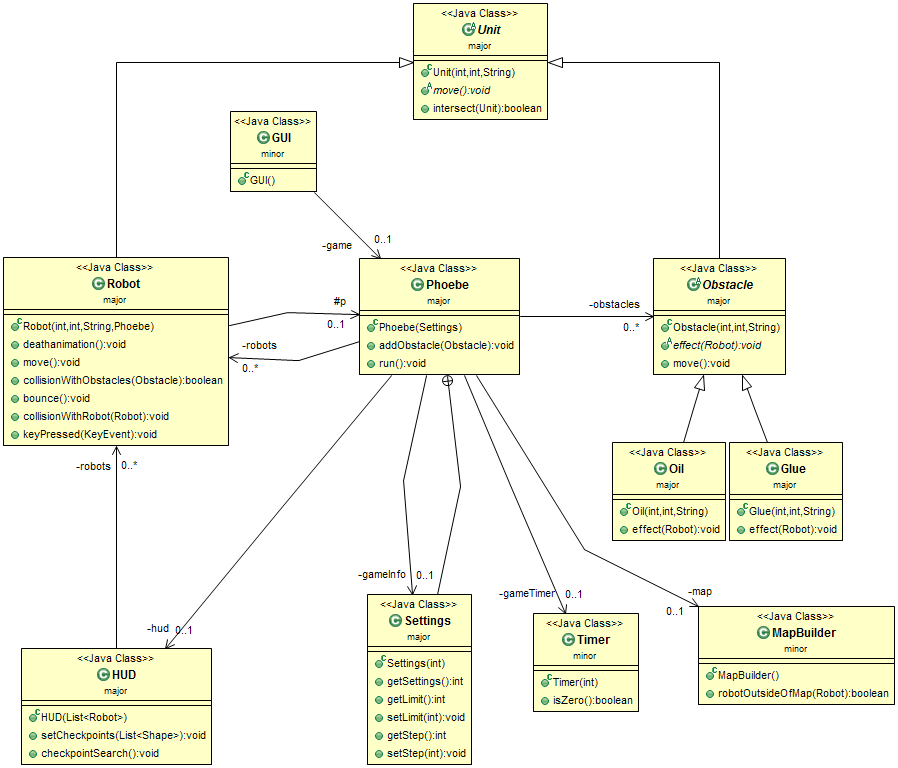
\includegraphics[width=17cm]{images/struktdiagram.PNG}
\caption{Osztálydiagram}
\label{fig:example3}
\end{center}
\end{figure}
\pagebreak

\section{Szekvencia diagramok}

\begin{figure}[h]
\begin{center}
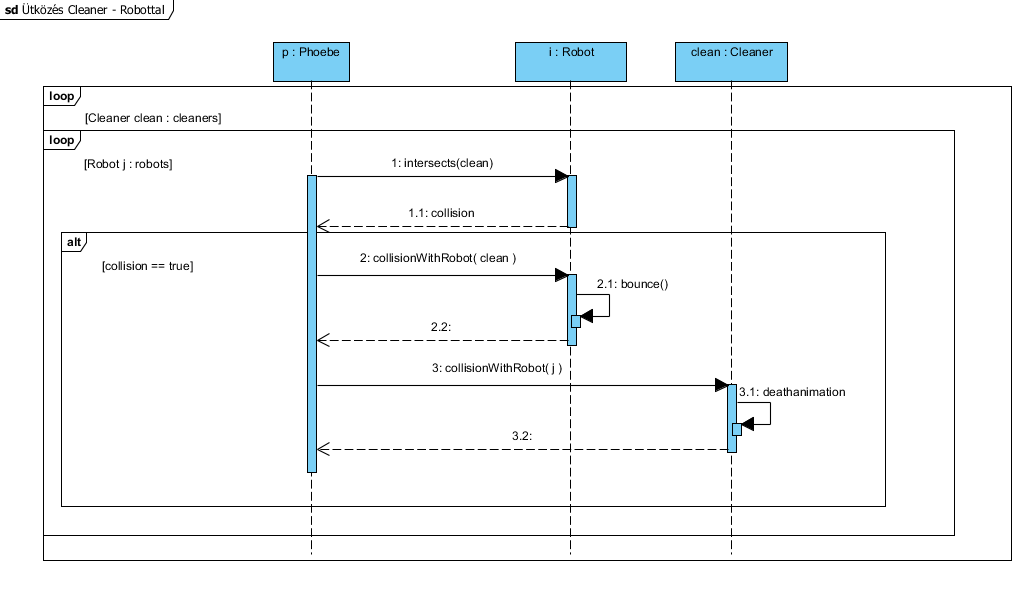
\includegraphics[width=17cm]{images/Szekvencia_diagrammok/collisionCleanerWithRobot()_sequence.PNG}
\caption{Robot ütközése takarító robottal}
\label{fig:example3}
\end{center}
\end{figure}
\pagebreak

\begin{figure}[h]
\begin{center}
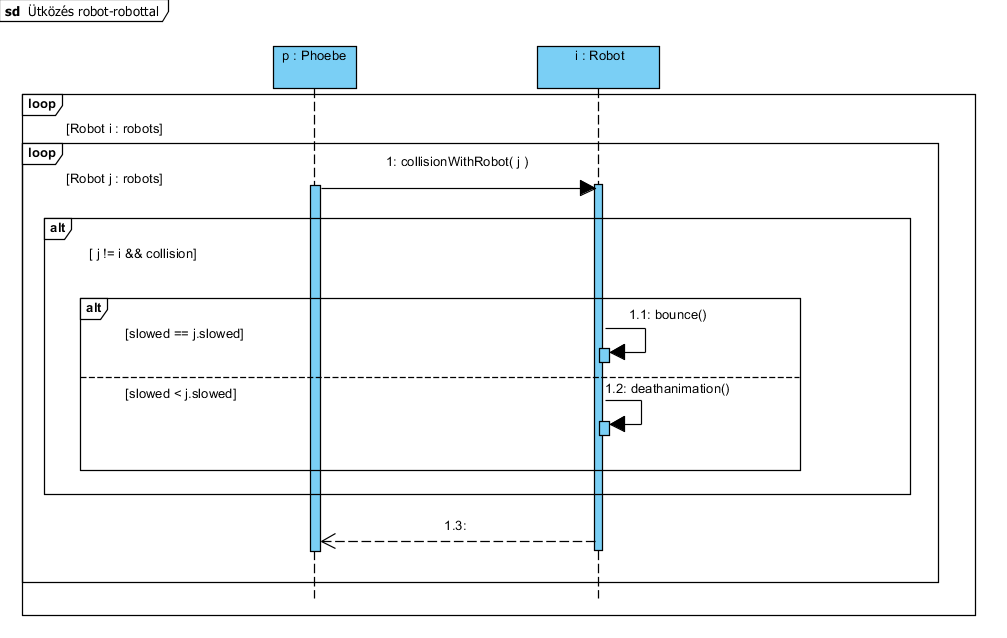
\includegraphics[width=17cm]{images/Szekvencia_diagrammok/collisionRobotWithRobot()_sequence.PNG}
\caption{Robot ütközése másik robottal}
\label{fig:example3}
\end{center}
\end{figure}
\pagebreak

\begin{figure}[h]
\begin{center}
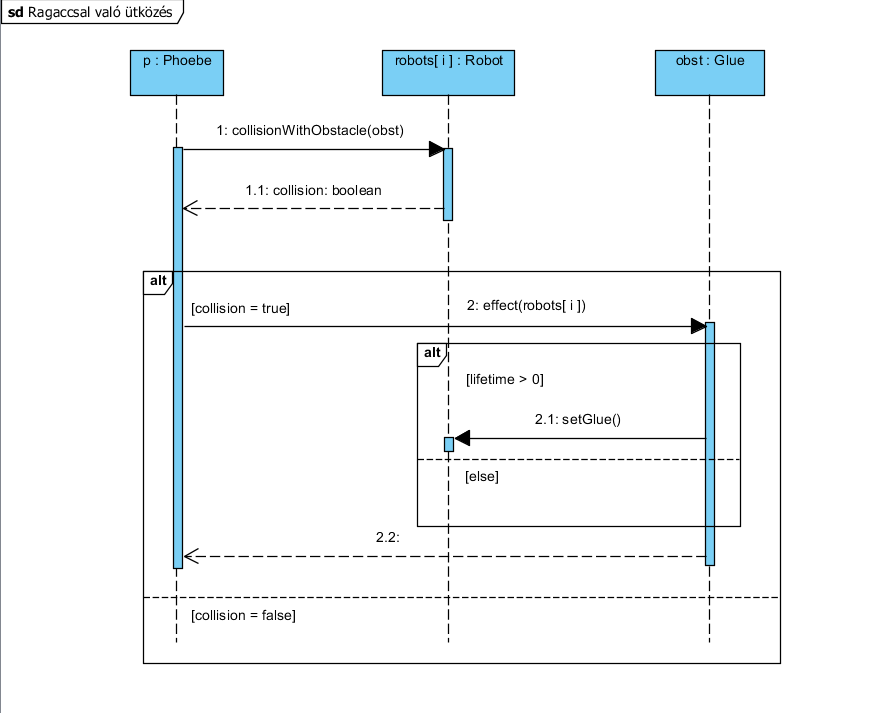
\includegraphics[width=17cm]{images/Szekvencia_diagrammok/collisionWithGlue()_sequence.PNG}
\caption{Robot ütközése ragaccsal}
\label{fig:example3}
\end{center}
\end{figure}
\pagebreak

\begin{figure}[h]
\begin{center}
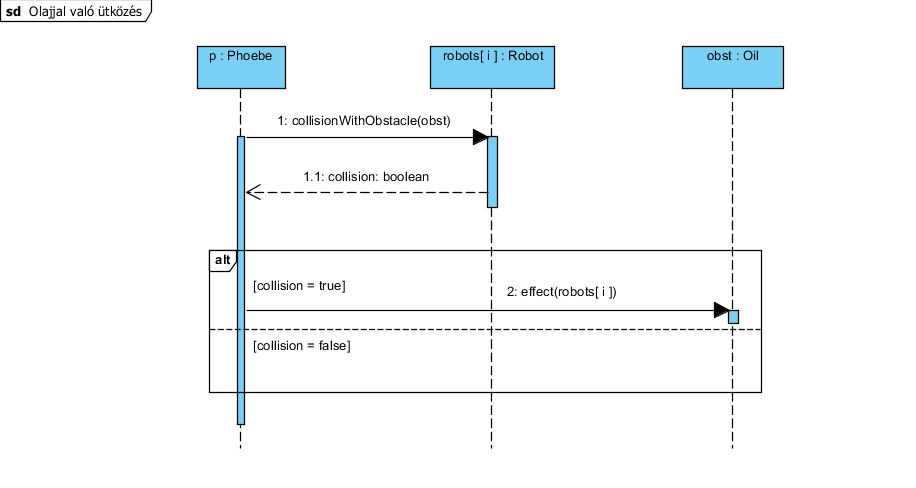
\includegraphics[width=17cm]{images/Szekvencia_diagrammok/collisionWithOil()_sequence.PNG}
\caption{Robot ütközése olajjal}
\label{fig:example3}
\end{center}
\end{figure}
\pagebreak

\setcounter{chapter}{6}
\chapter{Prototípus koncepciója}

\thispagestyle{fancy}

\section{Prototípus interface-definíciója}


\subsection{Az interfész általános leírása}
A prototípus csak a szabványos ki- és bemeneteket használja kommunikációra. Így az input fájlból is beolvasható, illetve az output fájlba is menthető. Ezáltal előre elkészített teszteseteket használva automatikusan is lehet tesztelni. Egy teszteset a prototípusnak adott parancsok sorozatából és az arra kapott kimenetből áll. Egy teszt sikeres, ha a kapott- és az elvárt kimenet megegyezik.

\subsection{Bemeneti nyelv}

\begin{itemize}
\item Glue <x> <y>
	\begin{itemize}
	\item Leírás: Ragacs létrehozása a pályán.
	\item Opciók: A ragacs (x,y) koordinátái.
	\end{itemize}
	
\item keyPressed <akadály\_gomb>
	\begin{itemize}
	\item Leírás: Akadály lerakása a robot koordinátáira.
	\item Opciók: 
	\begin{itemize}
    	    \item akadály\_gomb
        	    \begin{itemize}
        	        \item Up: Robot1 olaj lerakás
        	        \item Down: Robot1 ragacs lerakás
        	        \item W: Robot2 olaj lerakás
        	        \item S: Robot2 ragacs lerakás
        	    \end{itemize}
    	\end{itemize}
	\end{itemize}
	
\item keyPressed <irány\_gomb> <forgás értéke fokban>
	\begin{itemize}
	\item Leírás: A Robot következő irányának változtatása.
	\item Opciók: 
    	\begin{itemize}
    	    \item irány\_gomb
        	    \begin{itemize}
        	        \item Left: Robot1 balra forgatása
        	        \item Right: Robot1 jobbra forgatása
        	        \item A: Robot2 balra forgatása
        	        \item D: Robot2 jobbra forgatása
        	    \end{itemize}
        	 \item forgás érték = (0,180)
    	\end{itemize}
	\end{itemize}
	
\item listCleaners
	\begin{itemize}
	\item Leírás: A palyán lévő takarító kisrobotok kilistázása.
	\item Opciók: -
	\end{itemize}
	
\item listObstacles
	\begin{itemize}
	\item Leírás: Kilistázza a pályán lévő akadályokat.
	\item Opciók: -
	\end{itemize}
	
\item listRobots
	\begin{itemize}
	\item Leírás: Kilistázza a robotokat.
	\item Opciók: -
	\end{itemize}
	
\item MapBuilder 
	\begin{itemize}
	\item Leírás: Pálya betöltése a játékba.
	\item Opciók: Pálya kiválasztása.
	\end{itemize}
	
\item move
	\begin{itemize}
	\item Leírás: Robotok, Cleanerek mozgatása.
	\item Opciók: -
	\end{itemize}
	
\item Oil <x> <y>
	\begin{itemize}
	\item Leírás: Olajfolt létrehozása a pályán.
	\item Opciók: Az olajfolt (x,y) koordinátái.
	\end{itemize}
	
\item setCheckpoints
	\begin{itemize}
	\item Leírás: A pálya checkpointjainak a beállítása.
	\item Opciók: -
	\end{itemize}

\end{itemize}

\subsection{Kimeneti nyelv}

jelölés:<osztály tagváltozója>
\begin{itemize}
\item Robot: 
	\begin{itemize}
	\item ToString(): (nem írja ki automatikusan a szöveget csak visszaad egy stringet, amit a Phoebe run metódusában kell kiíratni)
	        \begin{itemize}
	\item "Robot [id=<id>,  slowed=<slowed>,oiled=<oiled>, x=<x>,y=<y> \\,nextx=<arrowendx>,\\nexty=<arrowendy>,alpha=<alpha>,width=<WIDTH>,height=<HEIGHT>,numGlue=<numGlue>,numOil=<numOil>]" 
	        \end{itemize}
	\item Keypressed(int k):
	       \begin{itemize}
	        \item "nextx ,nexty modified to:<arrowendx>,<arrowendy>"
            \item "new oil created at: <x>,<y>" ( ha volt olajunk és k == VK\_DOWN)
            \item "not enough oil"( ha nincs olajunk és k==VK\_DOWN)
            \item "new glue created at:<x>,<y>"(ha volt ragacsunk és k== VK\_UP)
            \item "not enough glue"( ha nincs ragacsunk és k==VK\_UP)
        
	       \end{itemize}
	 \item CollisionWithRobot(Robot robot2):
	       	
	        \begin{itemize}
	        \item  "there was a collision between this: <this.toString()> and this: <robot2.toString()>"
	        
	        \end{itemize}
    \item deathAnimation():
	        \begin{itemize}
	        \item  "This:<robot.toString()> died"
	        
	        \end{itemize}
	 \item CollisionWithObstacle(Obstacle o):
	       	
	        \begin{itemize}
	        \item  "there was a collision between this: <this.toString()> and this: <o.toString()>"
	        
	        \end{itemize}
	\end{itemize}
	
	
\item Oil:
	\begin{itemize}
	\item effect(robot r):
	        \begin{itemize}
	        \item  "you jumped into oil"
	        \end{itemize}
	\item toString():
	       \begin{itemize}
	        \item "Oil[x=<x>, y=<y>, Width=<WIDTH>, Height=<HEIGHT>, remainingturns=<Turnsremaining>]"
	       \end{itemize}
	\end{itemize}
\item Glue:
	\begin{itemize}
	\item effect(robot r):
	        \begin{itemize}
	        \item "you jumped into glue"
	        \end{itemize}
	\item toString():
	       \begin{itemize}
	        \item"Glue [x=<x>, y=<y>, Width=<WIDTH>, Height=<HEIGHT>,remaininglife=<Liferemaining>]";
	       \end{itemize}
	\end{itemize}

\item Cleaner:
	\begin{itemize}
	\item toString():
	       \begin{itemize}
	        \item "Cleaner[x=<x>, y=<y>, Width=<WIDTH>, Height=<HEIGHT>, State=<state>]"
	       \end{itemize}
	 \item CollisionWithRobot(Robot robot2):     
	        \begin{itemize}
	        \item  "there was a collision between this: <this.toString()> and this: <robot2.toString()>"
	        
	        \end{itemize}
	 \item cleanUp(Obstacle o):     
	        \begin{itemize}
	        \item  " this: <o.toString()> was cleaned up"
	        
	 \item deathAnimation():
	        \begin{itemize}
	        \item  "This:<Cleaner.toString()> died"
	        
	        \end{itemize}
	        
	        \end{itemize}
\item CollisionWithObstacle(Obstacle o):     
	        \begin{itemize}
	        \item  "there was a collision between this: <this.toString()> and this: <o.toString()>"
	        
	        \end{itemize}
	        
	\end{itemize}
\end{itemize}
\newpage

\section{Összes részletes use-case}

\usecase{chechpointSearch}
{A robot egy checkpointba ugrott.}
{Tesztelő}
{A program megnézi, hogy a robot olyan területre ugrott, ahol checkpoint található. Ha beleugrott, megnöveli a robot „checkpoint elérésének” számát.}

\usecase{collisionWithCleaner}
{Robot és kisrobot területe metszik egymást.}
{Tesztelő}
{Ha a metszet nem üres, akkor a kisrobot meghal.}

\usecase{collisionWithObstacles}
{Robot és akadály területe metszik egymást.}
{Tesztelő}
{Ha a metszet nem üres, akkor beállítja a robotot a kívánt hatásra.}

\usecase{collisionWithRobot}
{Robot és robot területe metszik egymást.}
{Tesztelő}
{Ha a metszet nem üres és ugyanakkora a sebességük, akkor lepattannak egymásról. Ha különböző a sebességük, akkor a lassabb meghal.
}

\usecase{effect}
{Akadály hatása a robotra.}
{Tesztelő}
{Ha robot akadályba lép, akkor az adott akadálynak megfelelő változtatás hajtódik végre a roboton.}
\newpage

\usecase{Glue}
{Ragacs létrehozása}
{Tesztelő}
{A tesztelő a pálya megadott koordinátáira ragacsot helyez el.}

\usecase{keyPressed}
{A robot koordinátáira akadályt tesz le.}
{Tesztelő}
{Robot ugrása előtt a tesztelő az adott gombbal akadályt rak le a robot helyére.}

\usecase{listCleaners}
{Kilistázza a kisrobotokat.}
{Tesztelő}
{Kiírja a kimenetre a játékban levő kisrobotokat.}

\usecase{listObstacles}
{Kilistázza az akadályokat.}
{Tesztelő}
{Kiírja a kimenetre a játékban levő akadályokat (ragacsokat és olajfoltokat).}

\usecase{listRobots}
{Kilistázza a robotokat}
{Tesztelő}
{Kiírja a kimenetre a játékban levő robotokat.}

\usecase{MapBuilder}
{Pálya betöltése}
{Tesztelő}
{A tesztelő által kiválasztott pálya betöltése.}

\usecase{Move}
{Robot irányának beállítása.}
{Tesztelő}
{Robot ugrása előtt a tesztelő beállítja a robot irányát az irányváltoztató gombokkal (0-180).}
\newpage

\usecase{Oil}
{Olajfolt létrehozása}
{Tesztelő}
{A tesztelő a pálya megadott koordinátáira olajfoltot helyez el.}

\usecase{robotOutsideOfMap}
{Robot kiugrik a pályáról.}
{Tesztelő}
{Ha a robot kiugrik a pályáról, akkor meghal.}

\usecase{setCheckpoints}
{Checkpointok beállítása}
{Tesztelő}
{Beállítja a pályára a checkpointokat.}

\pagebreak
\section{Tesztelési terv}

\teszteset{Mozgás}	{A robot mozgásának tesztelése.}	{Teszteli, hogy a robot mozgása után az előre megadott értékeknek megfelelően történik a mozgás (a mozgás után a megfelelő helyen van).}
\teszteset{Irányváltoztatás}	{A robot irányváltoztatásának tesztelése.}	{Teszteli, hogy a robot különböző irányok beállítása után is a megfelelő helyre ugrik.}
\teszteset{Ütközés}	{A robotok ütközésének tesztelése.}	{Teszteli, hogy a két robot ütközése után a megfelelő helyre pattannak-e, illetve hogy az objektumok határai helyesen működnek.}
\teszteset{Leesés}	{A robot leesésének tesztelése.}	{Teszteli, hogy a pálya szélén a robot megszűnik-e létezni.}
\teszteset{Checkpoint}	{A robot checkpoint-ba érésének tesztelése.}	{Teszteli a checkpoint-ba érést, illetve hogy a robotnak megfelelően változnak-e az értékei ilyen esetben.}
\teszteset{Olajba ugrás}	{A robot olajba ugrását teszteli.}	{Teszteli, hogy egy olajba ugrás alkalmával változnak-e a robot értékei, vizsgálja az ütközést.}
\teszteset{Ragacsba ugrás}	{A robot ragacsba ugrását teszteli.}	{Teszteli, hogy egy ragacsba ugrás alkalmával változnak-e a robot értékei, vizsgálja az ütközést.}
\teszteset{Olaj lerakás}	{Olaj lerakása a pályán.}	{Teszteli, hogy a lerakás után létrejött-e az olaj a pályán.}
\teszteset{Ragacs lerakás}	{Ragacs lerakása a pályán.}	{Teszteli, hogy a lerakás után létrejött-e a ragacs a pályán.}
\teszteset{Olaj hatás}	{Az olaj hatását teszteli.}	{Teszteli, hogy olajos állapotban a robot képes-e irányt változtatni.}
\teszteset{Ragacs hatás}	{A ragacs hatását teszteli.}	{Teszteli, hogy ragacsos állapotban a robot milyen távolságra képes ugrani.}

\section{Tesztelést támogató segéd- és fordítóprogramok specifikálása}

Az egyes tesztesetek futtatásához a JUnit tesztelő keretrendszert használjuk. A segédprogram egy-egy teszthez tárolja a bemeneteket illetve az adott bemenethez várt kimenetet. A segédprogram lefuttatja a megadott teszteket, és összeveti a kimenetüket az előre definiált elvárt kimenettel. Ha a teszt kimenete nem egyezik meg az elvárt kimenettel, akkor a teszt nem sikerült, ellenkező esetben a teszt sikeres. Hiba esetén a segédprogram megjeleníti, hogy hol talált eltérést.

